%%%%%%%%%%%%%%%%%%%%%%%%%%%%%%%%%%%%%%%%%%%%%%%%%%%%%%%%%%%%%%%%%%%%%%%%%%%%%%%%
% test.tex
%%%%%%%%%%%%%%%%%%%%%%%%%%%%%%%%%%%%%%%%%%%%%%%%%%%%%%%%%%%%%%%%%%%%%%%%%%%%%%%%
%
% Authors:
% - pvincent
% - rdavid
%
% Contributors:
% - Unknown for now
%
%%%%%%%%%%%%%%%%%%%%%%%%%%%%%%%%%%%%%%%%%%%%%%%%%%%%%%%%%%%%%%%%%%%%%%%%%%%%%%%%


\documentclass{42-en}

% Handmade paralist package
% for more compact list

\newenvironment{ft_itemize}
{ \begin{itemize}
	\setlength{\itemsep}{0pt}
	\setlength{\parskip}{0pt}
	\setlength{\parsep}{0pt}     }
{ \end{itemize}                  }

%%%%%%%%%%%%%%%%%%%%%%%%%%%%%%%%%%%%%%%%%%%%%%%%%%%%%%%%%%%%%%%%%%%%%%%%%%%%%%%%
% Prologue
%%%%%%%%%%%%%%%%%%%%%%%%%%%%%%%%%%%%%%%%%%%%%%%%%%%%%%%%%%%%%%%%%%%%%%%%%%%%%%%%

\begin{document}


%Table des matieres

\title{OpenGL Project}

\subtitle{HumanGL}

\member {42 staff}{staff@42.fr}

\summary
{
  You like matrices ? Hmm... but do they like YOU ? \\
  After this project, you'll know both answers.
}

\maketitle

\tableofcontents

% Valeurs utilisees pour la generation de headers d'exercices
\turnindir{svn+ssh://rendus@rendus.42.fr/sujetdetest-2142-login\_x}

\newpage

%%%%%%%%%%%%%%%%%%%%%%%%%%%%%%%%%%%%%%%%%%%%%%%%%%%%%%%%%%%%%%%%%%%%%%%%%%%%%%%%
% Start document
%%%%%%%%%%%%%%%%%%%%%%%%%%%%%%%%%%%%%%%%%%%%%%%%%%%%%%%%%%%%%%%%%%%%%%%%%%%%%%%%

\chapter{Foreword}
{
	These are the lyrics of September by Earth, Wind and Fire :\\
	\\
	\small
		Do you remember the 21st night of September?\\
		Love was changing the mind of pretenders\\
		While chasing the clouds away\\
		\\
		Our hearts were ringing\\
		In the key that our souls were singing.\\
		As we danced in the night,\\
		Remember - how the stars stole the night away, yeah yeah yeah.\\
		\\
		Hey hey hey,\\
		Ba de ya - say do you remember\\
		Ba de ya - dancing in September\\
		Ba de ya - never was a cloudy day\\
		\\
		Ba duda, ba duda, ba duda, badu\\
		Ba duda, badu, ba duda, badu\\
		Ba duda, badu, ba duda\\
		\\
		My thoughts are with you\\
		Holding hands with your heart to see you\\
		Only blue talk and love,\\
		Remember - how we knew love was here to stay\\
		\\
		Now December found the love that we shared in September.\\
		Only blue talk and love,\\
		Remember - the true love we share today\\
		\\
		Hey hey hey\\
		Ba de ya - say do you remember\\
		Ba de ya - dancing in September\\
		Ba de ya - never was a cloudy day....there was a\\
		Ba de ya - say do you remember\\
		Ba de ya - dancing in September\\
		Ba de ya - golden dreams were shiny days\\
		\\
		Now our bell was ringing, aha\\
		Our souls were singing.\\
		Do you remember every cloudy day - yau !\\
		\\
		There was a\\
		Ba de ya - say do you remember\\
		Ba de ya - dancing in September\\
		Ba de ya - never was a cloudy day....there was a\\
		Ba de ya - say do you remember\\
		Ba de ya - dancing in September\\
		Ba de ya - golden dreams were shiny days\\
		\\
		Ba de ya de ya de ya\\
		Ba de ya de ya de ya\\
		Ba de ya de ya de ya - De ya.... {x2}\\
		\\
		\\
		\\
		\\
		This subject won't be easier if you are listening Disco, but that's freakin' cool.\\
		And if you're feeling bad about some difficulties, just think about Travolta.\\
}

\newpage
	\chapter{Introduction}

		In this project, you must implement a skeletal animation (also called 'Rigging') with a hierarchical model. In order to achieve that you will need to implement your very own matrices and matrix stack.\\
		\\

\newpage
	\chapter{The project}
		\section{Mendatory part}
		Body parts should be correctly articulated using your own matrix stack implementation. For example, if the torso rotate, all the members must follow accordingly, therefore if the upper arm move only the forearm have to follow. When you modify the size of a member, related parts automatically reposition themself.\newline
		Your model will have the following parts :
		\begin{ft_itemize}
			\item a head
			\item a torso
			\item two arms with
			\begin{ft_itemize}
				\item upper arm
				\item forearm
			\end{ft_itemize}
			\item two legs with
			\begin{ft_itemize}
				\item thigh
				\item lower part
			\end{ft_itemize}
		\end{ft_itemize}
		{
			\noindent
			It should be able to walk, jump and stay put.
		}
		\begin{figure}[ht!]
			\centering
				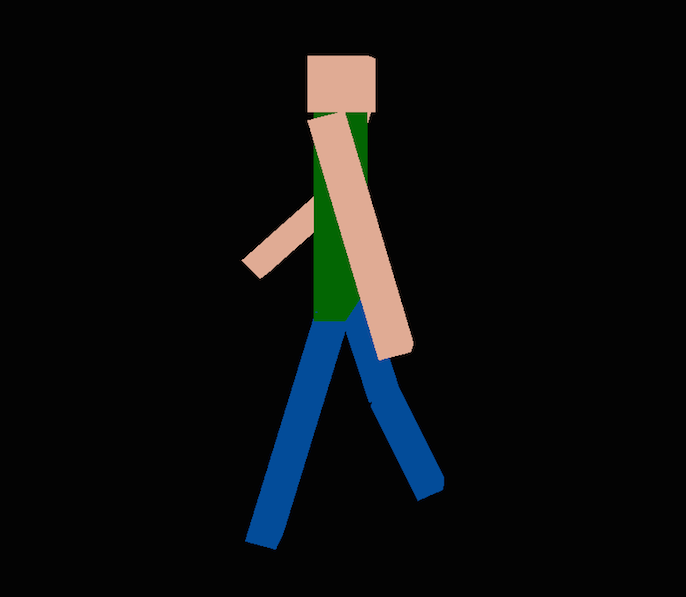
\includegraphics[width=90mm]{images/humangl-walking.png}
		\end{figure}
\newpage
	\section{Constraints}
		The following constraints have to be respected in order to have points.
		\subsection{Realisation}
            You must implement all the matrix stuff (matrices, matrix stack, transformations...).\\
            \\
			Each body part will be drawn by one and only one function call. This function will draw a 1x1x1 geometric shape at the origin of the current matrix.
		\\
		\info
		{
			Upper and lower part of the same member are indeed two different parts.
		}
		\
		\subsection{Language}
            You must use OpenGL; modern OpenGL: 4.0 minimum, shaders are of course not an option.\\
            \\
			A makefile or something similar is required. Only what contains your repository will be evaluated.\\
			\\
			You can use the graphic library of your choice (MLX, GLFW, SDL2, SFML...) but you can't use libraries that do the job for you. For exemple, GLM-like libraries will result in 0 points.\\
			\\
			You are free to use whatever language you want. If you use C, you have to respect the Norm, as usual.\\

		\newpage
			\section{Bonuses}

			When your hierarchical model is completely working, it will be easy to add :
			\begin{itemize}
				\item More body parts.
				\item Other move patterns (Disco dance, Kung-fu fighting, ...).
				\item A kick-ass graphic interface where you can for example modify body part size, change their color, etc...
			\end{itemize}
			\
			\\
			There will be some points dedicated to these bonuses and some more for your creativity.



\newpage
	\chapter {Defense sessions}
		Be prepared to :
		\begin{itemize}
			\item Obviously run the program and show the different move patterns.
			\item Change member sizes.
			\item Show your drawing function, his calls and explain how it works.
			\item Explain your hierarchical model and the resulting matrix stack.
		\end{itemize}

%%%%%%%%%%%%%%%%%%%%%%%%%%%%%%%%%%%%%%%%%%%%%%%%%%%%%%%%%%%%%%%%%%%%%%%%%%%%%%%%
% End document
%%%%%%%%%%%%%%%%%%%%%%%%%%%%%%%%%%%%%%%%%%%%%%%%%%%%%%%%%%%%%%%%%%%%%%%%%%%%%%%%

\end{document}

